% !TEX program = xelatex
% =============================================================================
%  并行处理课程大作业报告 —— TSMM 高性能优化
%  编译方式：xelatex report.tex  (需两次以生成目录与交叉引用)
%  依赖：ctex, booktabs, listings, amsmath, amssymb, geometry, hyperref,
%        tikz, xcolor, array, caption, fancyhdr
%  说明：本文档使用 ctexart 文档类与 XeLaTeX，中文字体采用开源 Fandol 字体，
%        排版风格对齐课程提供的《课程报告.pdf》模板。
% =============================================================================
\documentclass[11pt,a4paper,fontset=fandol]{ctexart}

% ---------- 页面与字体 ----------
\usepackage[a4paper,left=2.6cm,right=2.6cm,top=2.8cm,bottom=2.6cm]{geometry}
\usepackage{amsmath,amssymb,amsfonts}
\usepackage{booktabs}
\usepackage{array}
\usepackage{longtable}
\usepackage{multirow}
\usepackage{graphicx}
\usepackage{xcolor}
\usepackage{caption}
\usepackage{float}
\usepackage{enumitem}
\usepackage{listings}
\usepackage{tikz}
\usetikzlibrary{shapes.geometric,arrows.meta,positioning,calc}
\usepackage{fancyhdr}
\usepackage[colorlinks=true,linkcolor=black,citecolor=blue,urlcolor=blue,
            bookmarksnumbered=true]{hyperref}

% ---------- 中文字体设置（使用开源 Fandol 字体，由 fontset=fandol 提供）----------
% ctex 在 fontset=fandol 下已自动定义 \songti \heiti \kaiti \fangsong 等命令，
% 直接使用即可，无需重复定义。

% ---------- 标题样式 ----------
\ctexset{
  section/format   = {\Large\heiti\raggedright},
  subsection/format= {\large\heiti\raggedright},
  subsubsection/format = {\normalsize\heiti\raggedright},
}

% ---------- 表格题注 ----------
\captionsetup[table]{labelsep=quad,font=small,name=表}
\captionsetup[figure]{labelsep=quad,font=small,name=图}
\renewcommand{\arraystretch}{1.25}

% ---------- 代码清单样式 ----------
\definecolor{codebg}{RGB}{248,248,248}
\definecolor{codecomment}{RGB}{0,128,0}
\definecolor{codekeyword}{RGB}{0,0,200}
\definecolor{codestring}{RGB}{170,55,55}
\definecolor{coderule}{RGB}{220,220,220}
\lstset{
  basicstyle=\ttfamily\small,
  backgroundcolor=\color{codebg},
  commentstyle=\color{codecomment},
  keywordstyle=\color{codekeyword}\bfseries,
  stringstyle=\color{codestring},
  numberstyle=\tiny\color{gray},
  numbers=left,
  numbersep=8pt,
  frame=single,
  rulecolor=\color{coderule},
  breaklines=true,
  breakatwhitespace=true,
  showstringspaces=false,
  tabsize=2,
  columns=fullflexible,
  keepspaces=true,
  xleftmargin=2em,
  framexleftmargin=1.5em,
  language=C++,
  extendedchars=true,
  literate={’}{{'}}1 {…}{{...}}3,
  escapeinside={(*@}{@*)},
}
\lstdefinestyle{bashstyle}{language=bash,keywordstyle=\color{codekeyword}\bfseries}
\lstdefinestyle{plainstyle}{language=,numbers=none,commentstyle=\color{black}}

% ---------- 页眉页脚 ----------
\pagestyle{fancy}
\fancyhf{}
\fancyhead[L]{\small\heiti TSMM 高性能优化}
\fancyhead[R]{\small\thepage}
\renewcommand{\headrulewidth}{0.4pt}

% ---------- TikZ 样式 ----------
\tikzset{
  decision/.style={rectangle,rounded corners,draw=black!70,fill=blue!5,
                   text width=6.5em,align=center,minimum height=2.6em,font=\small},
  leaf/.style={rectangle,rounded corners,draw=black!70,fill=green!8,
               text width=5.6em,align=center,minimum height=3.0em,font=\scriptsize,inner sep=3pt},
  zmm/.style={rectangle,draw=black!60,fill=orange!10,minimum width=3.2em,
              minimum height=2.0em,align=center,font=\footnotesize},
  arr/.style={-{Stealth[length=2mm]},draw=black!70},
}

\begin{document}

% =============================================================================
%  标题页
% =============================================================================
\begin{titlepage}
\centering
\vspace*{2.2cm}
{\heiti\Huge 并行处理课程大作业报告\par}
\vspace{1.4cm}
{\heiti\LARGE Tall-Skinny Matrix Multiplication\par}
\vspace{0.4cm}
{\heiti\LARGE (TSMM) 高性能优化\par}
\vspace{0.9cm}
{\heiti\large ——基于形状感知调度的 AVX-512 多版本内核与自动调优方案\par}
\vfill
{\large
\begin{tabular}{rl}
\heiti 姓名： & 魏照峰 \\[4pt]
\heiti 学号： & 2025E8013282017 \\[4pt]
\heiti 单位： & 中国科学院计算技术研究所 \\[4pt]
\heiti 日期： & 2026 年 6 月 25 日 \\
\end{tabular}\par}
\vspace{1.6cm}
{\small 目标平台：Intel Xeon Platinum 9242（96 核，4 NUMA）@ BSCC bscc-t6\par}
\vspace{2.2cm}
\end{titlepage}

% =============================================================================
%  目录
% =============================================================================
\thispagestyle{empty}
\tableofcontents
\newpage

% =============================================================================
\section{项目背景与作业要求}

\subsection{问题定义}
Tall-Skinny Matrix Multiplication (TSMM) 指如下矩阵运算：
\begin{equation}
C = A^{T} \times B
\end{equation}
其中 $A \in \mathbb{R}^{k \times m}$，$B \in \mathbb{R}^{k \times n}$，$C \in \mathbb{R}^{m \times n}$，三个矩阵均为双精度（FP64）稠密矩阵。展开来看，输出矩阵的每个元素是 $A$ 的第 $i$ 列与 $B$ 的第 $j$ 列在归约维度 $k$ 上的内积：
\begin{equation}
C[i,j] = \sum_{p=0}^{k-1} A[p,i]\cdot B[p,j] = \langle \vec{a}_i, \vec{b}_j \rangle
\end{equation}

这一运算广泛出现在科学计算场景中：第一性原理计算（VASP）的波函数投影、深度学习注意力机制的 $QK^{T}$、有限元分析的刚度矩阵组装、EDA 电路仿真等。

TSMM 区别于通用 GEMM 的核心特点是\textbf{矩阵形状极端且多样}——归约维度 $k$ 可能极大（数十万）或极小（十几），$m$ 与 $n$ 的比值可能跨越数个数量级。这种“高瘦/矮胖”的形状多样性使得任何单一的通用 GEMM 优化策略都无法在所有场景下达到最优，必须针对不同形状设计差异化的优化方案——这正是本项目的核心动机。

\subsection{作业要求}
课程大作业分为两个阶段：
\begin{enumerate}[leftmargin=2.4em]
  \item \textbf{阶段一（基础）}：串行 C/C++ 实现，支持行主序与列主序两种数据布局，与 BLAS 库（MKL/OpenBLAS）对比，建立性能模型并用工具分析瓶颈；
  \item \textbf{阶段二（优化）}：OpenMP 多线程并行 + Cache Blocking + 访存优化 + 调度策略对比，最终与 MKL 进行性能对标。
\end{enumerate}

\subsection{测试用例}
课程指定了 4 个必选（required）和 4 个可选（optional）测试用例，覆盖了从“大输出小 $k$”到“极小输出极大 $k$”的全部典型形状。

\begin{table}[H]
\centering
\caption{TSMM 测试用例}
\small
\begin{tabular}{ccrrrrrl}
\toprule
类别 & Case & $m$ & $n$ & $k$ & 总 FLOPs & 输出元素 & 形状特征 \\
\midrule
required & T1 & 4000 & 16000 & 128 & $1.64\!\times\!10^{10}$ & 64{,}000{,}000 & 大输出，$k$ 中等 \\
required & T2 & 8 & 16 & 16000 & $4.10\!\times\!10^{6}$ & 128 & 极小输出，$k$ 极大 \\
required & T3 & 32 & 16000 & 16 & $1.64\!\times\!10^{7}$ & 512{,}000 & $k$ 极小，$n$ 极长 \\
required & T4 & 144 & 144 & 144 & $5.97\!\times\!10^{6}$ & 20{,}736 & 中小方阵 \\
optional & O1 & 16 & 12344 & 16 & $6.32\!\times\!10^{6}$ & 197{,}504 & $k$ 小，$n$ 较大 \\
optional & O2 & 4 & 64 & 606841 & $3.11\!\times\!10^{8}$ & 256 & 输出极小，$k$ 极大 \\
optional & O3 & 442 & 193 & 11 & $1.88\!\times\!10^{6}$ & 85{,}306 & $k$ 极小，输出中等 \\
optional & O4 & 40 & 1127228 & 40 & $3.61\!\times\!10^{9}$ & 45{,}089{,}120 & $n$ 极大，$k$ 小 \\
\bottomrule
\end{tabular}
\end{table}

四种必选用例分别考验不同的优化维度：
\begin{itemize}[leftmargin=2.4em]
  \item \textbf{T1（大输出）}：考验大输出矩阵的计算吞吐、cache 复用与寄存器分块效率；
  \item \textbf{T2（极小输出大 $k$）}：考验输出并行度不足时如何沿 $k$ 维暴露并行；
  \item \textbf{T3（小 $k$ 长 $n$）}：考验大量短内积下的向量化与调度开销控制；
  \item \textbf{T4（中小方阵）}：考验中小规模下的多核扩展与同步开销平衡。
\end{itemize}

\subsection{实验平台}
实验在 BSCC 集群 \texttt{bscc-t6} 节点上完成，配置如下。

\begin{table}[H]
\centering
\caption{实验平台配置}
\small
\begin{tabular}{ll}
\toprule
项目 & 配置 \\
\midrule
CPU & Intel Xeon Platinum 9242 (Cascade Lake-AP) @ 2.30 GHz \\
核心数 & 2 sockets $\times$ 48 cores = 96 cores（无超线程 SMT） \\
缓存 & L1d 32 KB/core，L2 1 MB/core，L3 $\sim$36 MB/NUMA（非包含式） \\
向量化 & AVX-512（512-bit zmm），32 个 ZMM 寄存器，双 FMA 端口 \\
NUMA & 4 个 domain：node0 (0--23)、node1 (24--47)、node2 (48--71)、node3 (72--95) \\
内存带宽 & 6 通道 DDR4/socket，$\sim$120 GB/s/socket（实测可用） \\
编译器 & Intel oneAPI icpx 2022.1（GCC 10.2.0 作为 fallback） \\
BLAS 库 & Intel oneAPI MKL 2022.1 \\
作业系统 & Slurm，节点独占（\texttt{-{}-exclusive}） \\
\bottomrule
\end{tabular}
\end{table}

理论双精度峰值估算：单核 AVX-512 每周期 2 条 FMA $\times$ 8 双精度 $\times$ 2（乘加）= 32 FLOP/cycle，单核 @ 2.30 GHz 约 73.6 GFLOPS，96 核理论上限约 7.07 TFLOPS。但 AVX-512 密集负载会触发降频，实际可达频率低于标称值。

\subsection{评测方法学}
\begin{table}[H]
\centering
\caption{正式评测协议}
\small
\begin{tabular}{ll}
\toprule
项目 & 设置 \\
\midrule
数据布局 & 列主序（col-major，自定义内核的主优化路径） \\
Warmup & 10 次（不计时，稳定 CPU 频率与缓存状态） \\
Repeat & 20 次（取平均耗时，降低系统噪声） \\
性能指标 & $\mathrm{GFLOPS} = 2mnk / \mathrm{time}$ \\
正确性基准 & MKL \texttt{cblas\_dgemm} \\
误差标准 & Frobenius 相对误差 $\|C_{\text{got}}-C_{\text{ref}}\|_F / \|C_{\text{ref}}\|_F$ \\
通过阈值 & \texttt{rel\_err < 1e-9} \\
数据生成 & 线性同余哈希，保证跨运行可复现 \\
\bottomrule
\end{tabular}
\end{table}

\textbf{为什么用 Frobenius 相对误差而非逐元素误差}：TSMM 结果中可能存在接近 0 的元素，逐元素相对误差会因分母趋零而误报；Frobenius 范数对整个矩阵做归一化，更稳健。

\textbf{关于主频、睿频与 Warmup}：Intel Xeon Platinum 9242 标称主频 2.30 GHz。轻负载下单核可通过睿频（Turbo Boost）短时提升至更高频率；但在 AVX-512 满负载、多核同时活跃时，由于功耗墙和散热限制，CPU 会降至 AVX-512 持续频率（通常低于标称值）。若不预热直接计时，前几次迭代会包含从低频爬升到稳定频率的过程，导致测量偏慢且方差大。因此正式测试前执行 10 次 warmup，使 CPU 进入稳定的 AVX-512 工作频率、数据进入缓存、OpenMP 线程池完成初始化，再取 20 次测量平均。

% =============================================================================
\section{代码架构设计}

\subsection{模块化组织}
整个项目采用“\textbf{算子与评测解耦}”的模块化设计：每个优化版本作为一个独立算子（op）实现统一的生命周期接口，由 benchmark 主程序统一驱动。新增优化版本无需改动 benchmark 逻辑，便于逐步实验、回滚和横向对比。

\begin{table}[H]
\centering
\caption{代码模块组织}
\small
\begin{tabular}{lll}
\toprule
模块 & 文件 & 功能 \\
\midrule
公共接口 & \texttt{include/tsmm.h} & Problem 定义、算子接口、Layout 枚举 \\
公共工具 & \texttt{include/common.h} & 对齐内存分配 \texttt{tsmm\_aligned\_alloc} 等 \\
v0 串行 & \texttt{ops/v0\_naive.cpp} & 三重循环基线（正确性参考 + 性能下界） \\
v1 分块 & \texttt{ops/v1\_blocked.cpp} & Cache blocking + MR$\times$NR 寄存器分块 \\
v2 OpenMP & \texttt{ops/v2\_openmp.cpp} & 输出 tile OpenMP 并行 \\
v3 AVX-512 & \texttt{ops/v3\_avx512.cpp} & AVX-512 形状分流内核（dot4 / outer8） \\
v4 k-reduce & \texttt{ops/v4\_kreduce.cpp} & $k$ 维并行归约（极小输出大 $k$） \\
v5 dot & \texttt{ops/v5\_smallk\_packa.cpp} & 输出点并行 dot 内核 \\
v6 smallk\_col & \texttt{ops/v6\_smallk\_col.cpp} & 超大 $n$ 小 $k$ packed-A 列核（带 gating） \\
BLAS 参考 & \texttt{ops/v9\_blas.cpp} & MKL/OpenBLAS 包装（正确性 oracle） \\
Benchmark & \texttt{benchmark.cpp} & 数据生成、计时、正确性验证、JSON 输出 \\
自动调优 & \texttt{run\_autotune.sh} & 线程/布局/调度扫描，NUMA 绑定 \\
结果汇总 & \texttt{scripts/summarize\_autotune.py} & 跨线程最优选择、MKL 对比 \\
\bottomrule
\end{tabular}
\end{table}

\subsection{统一算子接口}
每个算子实现三段式生命周期：
\begin{lstlisting}
struct TsmmOp {
    const char* name;
    const char* desc;
    void* (*prepare)(int m, int n, int k);              // 分配上下文/缓冲区
    void  (*compute)(const TsmmProblem& p, void* ctx);  // 计算 C = A^T B
    void  (*destroy)(void* ctx);                        // 释放
};
\end{lstlisting}
\texttt{prepare} 阶段分配的缓冲区（如 v4 的 partial C、v6 的 packed-A）不计入计时，确保 \texttt{compute} 计时只反映核心计算成本。这种分离让需要预分配的算子能与零分配算子公平对比。

\subsection{统一布局索引}
核心设计之一是\textbf{布局无关索引}。在列主序布局下，$A$ 的第 $i$ 列（即参与内积的 $\vec{a}_i$）和 $B$ 的第 $j$ 列都是长度为 $k$ 的\textbf{连续}数组。因此基础内积 \texttt{dot(A\_col\_i, B\_col\_j)} 是两个单位步长向量的点积，对硬件预取和 SIMD 自动向量化都极为友好。这是本项目选择列主序作为主优化路径的根本原因。行主序作为 fallback 保留，主要用于正确性交叉验证。

% =============================================================================
\section{阶段一：串行基线实现与分析}

\subsection{串行参考实现 v0\_naive}
串行版本严格按数学定义实现三重循环：
\begin{lstlisting}
for (int i = 0; i < m; ++i)
    for (int j = 0; j < n; ++j) {
        double sum = 0.0;
        for (int p = 0; p < k; ++p)
            sum += A[p * m + i] * B[p * n + j];
        C[i * n + j] = sum;
    }
\end{lstlisting}
在列主序路径下，内层退化为对两个连续 $k$ 向量的点积。该实现无 SIMD、无并行、无缓存分块，承担两个角色：(1) \textbf{正确性参考}——所有优化版本结果与之逐元素对比；(2) \textbf{性能下界}——衡量优化的绝对收益。

\subsection{性能基线}
\begin{table}[H]
\centering
\caption{串行基线性能（单线程，列主序）}
\small
\begin{tabular}{lrr}
\toprule
Case & GFLOPS & 占单核理论峰值 \\
\midrule
T1 & $\sim$6.6 & $\sim$9\% \\
T2 & $\sim$6.7 & $\sim$9\% \\
T3 & $\sim$7.3 & $\sim$10\% \\
T4 & $\sim$12.9 & $\sim$18\% \\
\bottomrule
\end{tabular}
\end{table}
串行实现仅达单核理论峰值的 9\%--18\%。性能损失来源于三个层面：(1) 无显式 SIMD，预期损失 4--8$\times$；(2) 无缓存分块，严重 memory-bound，预期损失 $\sim$10$\times$；(3) 无寄存器分块/循环展开/软件预取。

\subsection{Roofline 模型分析}
TSMM 总浮点操作数为 $\mathrm{FLOP} = 2mnk$，最小访存量约为 $\mathrm{Bytes} \approx 8(mk + nk + mn)$，算术强度：
\begin{equation}
\mathrm{AI} = \frac{2mnk}{8(mk + nk + mn)} \quad \text{(FLOP/Byte)}
\end{equation}
不分块时每个 $p$ 步都需重新加载 $A[p,i]$ 与 $B[p,j]$ 并读写 $C[i,j]$，有效算术强度仅约 0.125--0.25 FLOP/Byte，落在 Cascade Lake roofline 的 memory-bound 区。

\begin{table}[H]
\centering
\caption{算术强度与瓶颈分析}
\small
\begin{tabular}{lll}
\toprule
Case & 主要瓶颈 & 优化方向 \\
\midrule
T1 & Memory $\to$ Compute 边界 & blocking + AVX-512 + 全核并行 \\
T2 & 严重 Memory-bound（C 仅 128 元素） & $k$ 维归约 / 输出点 dot 并行 \\
T3 & 严重 Memory-bound（$k$ 太小） & 输出 tile 并行 + 静态调度 \\
T4 & Compute-bound（可放入 L2） & 输出 tile 并行 + 寄存器分块 \\
O2 & 极端 Memory-bound & $k$ 维归约 \\
O4 & Streaming（$n$ 极大） & AVX-512 连续访存 + NUMA interleave \\
\bottomrule
\end{tabular}
\end{table}

通过 cache blocking 将 C tile 保持在寄存器/L1 中，可将 T1 的有效算术强度提升一个数量级，跨越 memory$\to$compute 边界；而 T2/O2 这类输出极小的 shape 受限于 C 复用率，blocking 收益有限，必须转向 $k$ 维并行。

\subsection{MKL 跨线程基线扫描}
公平对比的前提是确定 MKL 的“真实最佳”性能。我们对 MKL 进行了\textbf{线程数 $\times$ 布局}的完整扫描（job 33801149，8 shape $\times$ 2 布局 $\times$ 8 线程档 = 128 组）。

\begin{table}[H]
\centering
\caption{MKL 跨线程最佳性能}
\small
\begin{tabular}{lrrc}
\toprule
Case & MKL 最佳 GFLOPS & 最佳线程 & 最佳布局 \\
\midrule
T1 & 3943.03 & 96 & row \\
T2 & 266.49 & 48 & row \\
T3 & 1326.01 & 96 & col \\
T4 & 630.16 & 24 & row \\
O1 & 709.57 & 24 & col \\
O2 & 240.17 & 96 & row \\
O3 & 207.26 & 8 & row \\
O4 & 832.96 & 96 & col \\
\bottomrule
\end{tabular}
\end{table}

这一扫描揭示了贯穿全项目的关键发现：\textbf{MKL 在不同 shape 上的最优线程数差异极大}（从 8 到 96），最优布局也各不相同。固定用 96 线程同布局对比，既会高估某些 shape 上 MKL 的弱点、也会掩盖手写内核在合适线程数下的竞争力。因此最终评测采用 “per-shape best thread + best layout” 作为基准。

% =============================================================================
\section{阶段二：并行优化路径（v1--v6）}

本节按优化迭代顺序，逐版本详述设计思路、关键代码与性能影响。

\subsection{优化链路总览}
\begin{table}[H]
\centering
\caption{TSMM 优化链路总览（各 shape 最佳 GFLOPS）}
\small
\begin{tabular}{clrrrrr}
\toprule
版本 & 关键技术 & T1 & T2 & T3 & T4 & O4 \\
\midrule
v0 & 串行三重循环 & 6.6 & 6.7 & 7.3 & 12.9 & --- \\
v1 & Cache Blocking & 19.1 & 29.4 & 16.9 & 38.1 & 20.1 \\
v2 & OpenMP 输出 tile 并行 & 1547 & 79 & 766 & 619 & 720 \\
v3 & AVX-512 形状分流内核 & 1674 & 165 & 568 & 365 & 858 \\
v4 & $k$ 维归约 & 153 & 108 & 130 & 118 & 144 \\
v5 & 输出点 dot 并行 & 454 & 219 & 255 & 351 & 470 \\
v6 & 小 $k$ 列核（gating） & 450 & 234 & 242 & 322 & 578 \\
\midrule
\textbf{最终} & \textbf{形状感知 + 线程调优} & \textbf{1674} & \textbf{234} & \textbf{766} & \textbf{619} & \textbf{858} \\
\bottomrule
\end{tabular}
\end{table}
\noindent\footnotesize 注：v1 为单线程；v2--v6 取各自最优线程数下的最佳值。粗体为各 shape 最终选用版本。\normalsize

\subsection{v1: Cache Blocking 与寄存器分块}
v1 在串行基础上引入 \textbf{MR$\times$NR 输出寄存器 tile} 与 \textbf{KC 维 cache blocking}。对一个 tile 内的 MR$\times$NR 个 $C[r,c]$ 同时沿 $k$ 维累加，使每个加载的 A/B 元素被复用 MR 或 NR 次。
\begin{lstlisting}
constexpr int MR = 4, NR = 4, KC = 256;
for (int kc = 0; kc < k; kc += KC) {
    const int kb = min(KC, k - kc);
    for (int jc = 0; jc < n; jc += NR)
        for (int ic = 0; ic < m; ic += MR) {
            double acc[MR][NR] = {{0}};
            const double* Acol = A + (size_t)ic * k + kc;
            const double* Bcol = B + (size_t)jc * k + kc;
            for (int i = 0; i < kb; ++i) {
                double av[MR], bv[NR];
                for (int a = 0; a < MR; ++a) av[a] = Acol[a*(size_t)k + i];
                for (int b = 0; b < NR; ++b) bv[b] = Bcol[b*(size_t)k + i];
                for (int a = 0; a < MR; ++a)
                    for (int b = 0; b < NR; ++b)
                        acc[a][b] += av[a] * bv[b];   // MR*NR 次 FMA / 步
            }
            for (int b = 0; b < NR; ++b)
                for (int a = 0; a < MR; ++a)
                    C[(size_t)(jc+b)*m + (ic+a)] += acc[a][b];
        }
}
\end{lstlisting}
核心收益：每个 $k$ 步加载 MR+NR=8 个元素，却产生 MR$\times$NR=16 次 FMA，计算访存比从串行的 $\sim$1:2 提升到 $\sim$2:1。

\begin{table}[H]
\centering
\caption{v1 Blocking vs v0 串行（单线程）}
\small
\begin{tabular}{lrrr}
\toprule
Case & v0 GFLOPS & v1 GFLOPS & 提升 \\
\midrule
T1 & 6.58 & 19.09 & 2.90$\times$ \\
T2 & 6.66 & 29.36 & 4.41$\times$ \\
T3 & 7.29 & 16.85 & 2.31$\times$ \\
T4 & 12.92 & 38.11 & 2.95$\times$ \\
O3 & 2.57 & 11.93 & 4.64$\times$ \\
\bottomrule
\end{tabular}
\end{table}
仅靠改善局部性与寄存器复用即获得约 3$\times$ 稳定收益。但单线程性能距硬件峰值仍差一个数量级，必须引入多线程。

\subsection{v2: OpenMP 输出 tile 并行}
由于 $C$ 的每个 $(i,j)$ 元素是独立内积，\textbf{按输出空间划分天然无写冲突}。v2 将 $(m,n)$ 的 MR$\times$NR tile 网格展平为一维迭代空间，用 OpenMP 分发：
\begin{lstlisting}
constexpr int MR = 8, NR = 4;
const int mt = (m + MR - 1) / MR;   // 行 tile 数
const int nt = (n + NR - 1) / NR;   // 列 tile 数
const long ntiles = (long)mt * nt;
#pragma omp parallel for schedule(runtime)
for (long t = 0; t < ntiles; ++t) {
    const int it = t % mt, jt = t / mt;
    micro_tile(A, B, C, m, k, it*MR, jt*NR, mb, nb);
}
\end{lstlisting}
设计要点：(1) 展平 tile 网格合并 $(m,n)$ 两维迭代空间增加并行度，对“M 大”和“N 大”两类形状都均衡；(2) 私有 \texttt{acc[MR][NR]} 在寄存器/栈累加，$k$ 结束才写回 C；(3) 通过 \texttt{OMP\_SCHEDULE} 切换调度——实测对 tile 成本均匀但数量巨大的 TSMM，\texttt{static} 消除调度开销且负载均衡，为最优。

\begin{table}[H]
\centering
\caption{v2 OpenMP 在最优线程下的关键结果}
\small
\begin{tabular}{lrrrl}
\toprule
Case & 最佳线程 & GFLOPS & vs MKL best & 备注 \\
\midrule
T3 & 96 & 765.58 & 0.577 & required 小 $k$ 长 $n$ 最佳 \\
T4 & 48 & 618.54 & 0.982 & required 中小方阵最佳 \\
O1 & 48 & 441.38 & 0.622 & optional 小 $k$ 大 $n$ 最佳 \\
O3 & 48 & 188.05 & 0.907 & optional 小 $k$ 中输出最佳 \\
\bottomrule
\end{tabular}
\end{table}
但 v2 对 T2/O2 这类 $m\times n$ 极小（128/256 元素）的形状效果有限——输出 tile 数远不足以喂满 96 核。

\subsection{v3: AVX-512 形状分流内核（核心优化）}
v3 是贡献最大的单项优化之一。核心思想是将一个 C 子 tile \textbf{全部保持在 ZMM 寄存器中}，跨整个 $k$ 维在寄存器中累加，热循环内完全不写 C 内存，$k$ 结束后一次性 store。这将 C 写内存次数从 $O(mnk)$ 降至 $O(mn)$。v3 提供两个互补的微内核，按形状分流：
\begin{itemize}[leftmargin=2.4em]
  \item \textbf{dot4（4$\times$4 连续内积）}：用 ZMM 向量化连续的 $k$ 维点积，适合大输出/大 $k$（T1/O4/T2/O2）；
  \item \textbf{outer8（8$\times$8 外积）}：消除水平求和，适合短 $k$/小输出（T3/T4/O3），但需 gather 读 A。
\end{itemize}

\subsubsection{dot4 寄存器布局}
dot4 用 16 个 ZMM 累加器持有 4$\times$4 个部分内积，每个 ZMM 存 8 个 $k$-lane 部分和（最后水平求和）：

\begin{figure}[H]
\centering
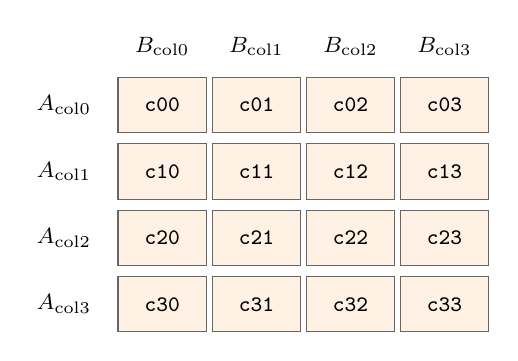
\begin{tikzpicture}[node distance=2pt]
  \foreach \r in {0,1,2,3} {
    \foreach \c in {0,1,2,3} {
      \node[zmm] (c\r\c) at (\c*3.4em, -\r*2.4em) {\texttt{c\r\c}};
    }
  }
  \node[above=4pt of c00] {\footnotesize $B_{\text{col}0}$};
  \node[above=4pt of c01] {\footnotesize $B_{\text{col}1}$};
  \node[above=4pt of c02] {\footnotesize $B_{\text{col}2}$};
  \node[above=4pt of c03] {\footnotesize $B_{\text{col}3}$};
  \node[left=6pt of c00] {\footnotesize $A_{\text{col}0}$};
  \node[left=6pt of c10] {\footnotesize $A_{\text{col}1}$};
  \node[left=6pt of c20] {\footnotesize $A_{\text{col}2}$};
  \node[left=6pt of c30] {\footnotesize $A_{\text{col}3}$};
\end{tikzpicture}
\caption{dot4 的 16 个 ZMM 累加器布局（每个含 8 个 $k$-lane 部分和）}
\end{figure}

\begin{lstlisting}
// dot4 主循环：每步加载 4 个 A 向量 + 4 个 B 向量，做 16 次 FMA
for (; i + 8 <= k; i += 8) {
    __m512d av0 = _mm512_loadu_pd(a0+i), ... , av3 = _mm512_loadu_pd(a3+i);
    __m512d bv0 = _mm512_loadu_pd(b0+i), ... , bv3 = _mm512_loadu_pd(b3+i);
    c00 = _mm512_fmadd_pd(av0, bv0, c00);   // 16 次独立 FMA
    c01 = _mm512_fmadd_pd(av0, bv1, c01);
    // ...
    c33 = _mm512_fmadd_pd(av3, bv3, c33);
}
r[x][y] = _mm512_reduce_add_pd(cxy);   // k 结束后水平求和写回
\end{lstlisting}

\subsubsection{outer8 设计与分流决策}
outer8 用 8 个 ZMM 累加器（每个对应一个 B 列、持有 8 行），每步广播 B 标量、gather 加载 A：
\begin{lstlisting}
const __m512i aidx = _mm512_set_epi64(7*k, 6*k, ... , 1*k, 0*k);
for (int i = 0; i < k; ++i) {
    const __m512d av = _mm512_i64gather_pd(aidx, abase + i, 8);  // gather A
    c0 = _mm512_fmadd_pd(av, _mm512_set1_pd(bbase[0*k+i]), c0);
    // ... c7
}
// 8 次向量 store，无水平求和
\end{lstlisting}
分流决策（阈值来自 Xeon 9242 实测）：
\begin{lstlisting}
static inline bool should_use_outer8(int m, int n, int k) {
    return (k <= 64 && n <= 20000) || (m <= 256 && n <= 256 && k <= 256);
}
\end{lstlisting}

\begin{table}[H]
\centering
\caption{v3 AVX-512 在最优线程下的关键结果}
\small
\begin{tabular}{llrrr}
\toprule
Case & 内核 & 最佳线程 & GFLOPS & vs MKL best \\
\midrule
T1 & dot4 & 96 & 1674.31 & 0.425 \\
O2 & dot4 & 24 & 117.22 & 0.488 \\
O4 & dot4 & 96 & \textbf{857.62} & \textbf{1.030} \\
\bottomrule
\end{tabular}
\end{table}
v3 在 T1 上达 1674 GFLOPS（T1 最佳手写内核），在 O4 上\textbf{超越 MKL 最佳 3\%}——是本项目的标志性成果。

\subsection{v4: $k$ 维并行归约}
T2（128 元素）、O2（256 元素）输出极小，输出 tile 并行最多产生几百个任务，96 核大量空转。必须沿\textbf{归约维度 $k$}暴露并行。v4 将 $k$ 区间切分给多个线程，每线程在私有 partial C 上累加自己的 $k$ 段，最后归约。线程数按 $k$ 自适应：
\begin{lstlisting}
static int choose_k_threads(int k, int max_threads) {
    int t = max(1, k / 1024);          // k=16000 -> ~16, k=606841 -> 96
    return min(max_threads, t);
}
#pragma omp parallel num_threads(use_threads)
{
    double* local = partials + tid * c_elems;
    const int k0 = (long long)k * tid / nt;     // 本线程 k 区间
    const int k1 = (long long)k * (tid+1) / nt;
    for (int c = 0; c < n; ++c)
        for (int r = 0; r < m; ++r)
            local[c*m + r] = dot_range(A+r*k, B+c*k, k0, k1);  // AVX-512 段内积
}
#pragma omp parallel for schedule(static)   // 跨线程归约 partial C -> C
for (long idx = 0; idx < c_elems; ++idx) {
    double sum = 0.0;
    for (int t = 0; t < use_threads; ++t) sum += partials[t*c_elems + idx];
    C[idx] = sum;
}
\end{lstlisting}
\textbf{护栏（guardrail）}：per-thread C 缓冲仅在 $m\times n$ 小时合理。\texttt{prepare} 阶段判断 $k\geq4096$ 且 $m\cdot n\leq65536$ 才启用 k-reduce，否则回退输出 tile 并行，避免为大输出 shape 分配巨大的 per-thread 矩阵。

v4 在 O2（$k=606841$）上从 v2 的几 GFLOPS 提升到 71+ GFLOPS（48t）。但在 T2 上 $k=16000$ 相对较小，归约开销占比偏高，最终不如 v5/v6。结论：\textbf{$k$ 维归约要求 $k$ 足够大以摊薄归约成本}。

\subsection{v5: 输出点并行 dot}
v5 的实验过程极具教训意义。最初尝试 small-k packed-A 预处理，但在 T3/O1 上出现严重退化（0.x GFLOPS）——packing 与微任务开销吞掉了全部收益。分析后\textbf{移除失败的 packA 路径}，保留其意外有效的 fallback：直接对每个输出元素并行计算连续内积：
\begin{lstlisting}
#pragma omp parallel for schedule(runtime)
for (long idx = 0; idx < (long)m * n; ++idx) {
    int r = idx % m, c = idx / m;
    const double* ap = A + (size_t)r * k;   // A 第 r 列，连续
    const double* bp = B + (size_t)c * k;   // B 第 c 列，连续
    double acc = 0.0;
    for (int i = 0; i < k; ++i) acc += ap[i] * bp[i];
    C[(size_t)c * m + r] = acc;
}
\end{lstlisting}
逻辑极简但鲁棒：当输出元素足够多以暴露并行、但 tiled 内核欠利用核心时（如 T2），它特别有效。T2 上从 v1 的 29.36 提升到 218.87 GFLOPS（48t）。

\subsection{v6: 超大 $n$ 小 $k$ 列核与 shape gating}
v6 尝试将 A 打包为 $k\times m$ 行连续布局，再按 B/C 列并行计算整列 C，对超大 $n$ 小 $k$ 形状（如 O4）友好：
\begin{lstlisting}
// 仅当 k<=64 && m<=512 && n>=100000 才启用 packing
ctx->enabled = (k <= 64 && m <= 512 && n >= 100000);
// packed-A 列核（AVX-512）：B 标量广播 x packed-A 向量
for (int c = 0; c < n; ++c)
    for (int rb = 0; rb < rb_count; ++rb) {
        __m512d acc = _mm512_setzero_pd();
        for (int i = 0; i < k; ++i) {
            __m512d av = _mm512_loadu_pd(packA + i*m + r0);
            __m512d bv = _mm512_set1_pd(bp[i]);
            acc = _mm512_fmadd_pd(av, bv, acc);
        }
        _mm512_storeu_pd(cp + r0, acc);
    }
\end{lstlisting}
\textbf{关键教训：shape gating 不可或缺}。第一次实测 v6 在 T3/O1/O3 上出现异常慢路径（packing 开销 $\gg$ 计算量）。最终加入严格门控：仅当 $n\geq100000$ 且 $k\leq64$ 且 $m\leq512$ 时启用 packed-A 列核，其余形状回退到输出点 dot。这样既保留了 O4/T2 的候选价值，又避免拖慢小形状。

\begin{table}[H]
\centering
\caption{v6 最佳结果}
\small
\begin{tabular}{lrrr}
\toprule
Case & 线程 & GFLOPS & vs MKL best \\
\midrule
T2 & 48 & \textbf{234.01} & \textbf{0.878} \\
O4 & 96 & 577.67 & 0.694 \\
\bottomrule
\end{tabular}
\end{table}
v6 在 T2 上达 234 GFLOPS，是 T2 的最佳手写内核。

% =============================================================================
\section{形状感知调度与自动调优框架}

\subsection{为什么不用单一“万能内核”}
前述六个内核各有擅长的形状区间，没有任何一个在全部 8 个 shape 上都最优。与其强行设计分支密布的万能内核，不如保留全部候选内核参与 benchmark，让\textbf{实测结果}为每个 shape 选择最优 (kernel, threads) 组合。决策逻辑如下图。

\begin{figure}[H]
\centering
\resizebox{\textwidth}{!}{%
\begin{tikzpicture}[x=1cm,y=1cm]
  % --- 节点（绝对坐标，间距大幅拉开，保证互不重叠且通透）---
  \node[decision] (in)    at ( 0    ,  0    ) {输入\\$(m,n,k)$};
  \node[decision] (small) at (-6.2  , -3.2  ) {输出 $m\!\cdot\!n$ 极小?};
  \node[decision] (large) at ( 6.2  , -3.2  ) {输出 $m\!\cdot\!n$ 大?};
  \node[leaf] (o2) at (-9.2  , -6.8 ) {O2:\\v4 kreduce\\(24--48t)};
  \node[leaf] (t2) at (-3.2  , -6.8 ) {T2:\\v6/v5 dot\\(48t)};
  \node[leaf] (o4) at ( 3.2  , -6.8 ) {O4:\\v3 dot4\\(96t, 超MKL)};
  \node[leaf] (t1) at ( 9.2  , -6.8 ) {T1:\\v3 dot4\\(96t)};
  \node[leaf] (v2) at ( 6.2  , -10.4) {T3/T4/O1/O3:\\v2 openmp\\(48--96t)};
  % --- 连线 ---
  \draw[arr] (in) -- (small);
  \draw[arr] (in) -- (large);
  \draw[arr] (small) -- (o2) node[pos=0.55,left,font=\scriptsize]{$k$ 极大};
  \draw[arr] (small) -- (t2) node[pos=0.55,right,font=\scriptsize]{$k$ 中等};
  \draw[arr] (large) -- (o4) node[pos=0.55,left,font=\scriptsize]{$n$ 极大};
  \draw[arr] (large) -- (t1) node[pos=0.55,right,font=\scriptsize]{常规};
  \draw[arr] (large) -- (v2) node[pos=0.62,right,font=\scriptsize]{小 $k$};
\end{tikzpicture}%
}
\caption{形状感知内核调度决策树}
\end{figure}

\subsection{自动调优脚本 run\_autotune.sh}
\texttt{run\_autotune.sh} 扫描线程数 $\times$ 布局 $\times$ 调度三个维度，并为每档线程数施加与 MKL 基线\textbf{完全一致}的 NUMA 绑定策略：
\begin{lstlisting}[style=bashstyle]
bind_cmd() {
    local t="$1"
    if   [ "$t" -le 24 ]; then echo "numactl --cpunodebind=0 --membind=0"
    elif [ "$t" -le 48 ]; then echo "numactl --cpunodebind=0-1 --interleave=0-1"
    else                       echo "numactl --cpunodebind=0-3 --interleave=all"
    fi
}
export OMP_PROC_BIND=spread; export OMP_PLACES=cores
export MKL_DYNAMIC=FALSE;    export KMP_AFFINITY=granularity=fine,compact,1,0
\end{lstlisting}
绑定策略：1--24 线程绑定 node0（单 NUMA，避免远程访存）；48 线程 interleave node0-1（双 NUMA）；96 线程 interleave 全部 4 个 node。

\textbf{经验教训}：\texttt{KMP\_AFFINITY} 优先级高于 \texttt{OMP\_PROC\_BIND}，二者冲突时以前者为准；运行时会有 OMP\_PLACES 被忽略的 warning，但绑定经 KMP\_AFFINITY 正确生效。

\textbf{默认只扫 col 布局}：早期默认扫描 row+col $\times$ static+dynamic，导致单次作业 $>$3h——某些专用内核（v5/v6）在 row-major 下未优化甚至 FAIL，O4 行主序路径极慢。最终将默认收敛为“col + static”，row/dynamic 改为显式 opt-in。

\subsection{结果汇总 summarize\_autotune.py}
\texttt{scripts/summarize\_autotune.py} 聚合所有线程档的 JSON 结果，为每个 shape 选出最快的正确算子组合，与 MKL 跨线程基线 CSV 对比，计算 required / all 两组几何平均加速比，输出 \texttt{autotune\_summary.csv}。

% =============================================================================
\section{最终性能结果}
正式评测：job \textbf{33823781}，参数 \texttt{warmup=10, repeat=20, layout=col, schedule=static}，线程扫描 $\{1,2,4,8,16,24,48,96\}$。

\subsection{线程扩展性曲线}
\begin{table}[H]
\centering
\caption{各线程数下 required / all geomean（vs 同线程 MKL）}
\small
\begin{tabular}{crr}
\toprule
线程数 & required geomean & all geomean \\
\midrule
1 & 0.574 & 0.547 \\
2 & 0.507 & 0.551 \\
4 & 0.512 & 0.541 \\
8 & 0.594 & 0.624 \\
16 & 0.654 & 0.727 \\
24 & 0.707 & 0.764 \\
48 & \textbf{1.004} & 0.992 \\
96 & \textbf{1.054} & 0.848 \\
\bottomrule
\end{tabular}
\end{table}
48 线程是手写内核的“甜点”区——相对同线程 MKL 已反超（1.004$\times$）。96 线程时 required 进一步升至 1.054$\times$，但 all 反而回落到 0.848$\times$，因为 O2/O3 等小形状在 96 线程下因 NUMA 跨节点开销而退化。这正是后续 per-shape 线程调优的依据。

\subsection{required shape 线程扩展明细}
\begin{table}[H]
\centering
\caption{required shape 各线程数 GFLOPS}
\small
\begin{tabular}{crrrr}
\toprule
线程 & T1 (v3) & T2 (best) & T3 (v2) & T4 (v2) \\
\midrule
1 & 21.7 & 29.8 & 20.9 & 48.6 \\
8 & 170.8 & 207.3 & 151.1 & 297.7 \\
16 & 308.9 & 204.0 & 273.6 & 507.0 \\
24 & 395.9 & 209.5 & 365.3 & 591.4 \\
48 & 844.8 & 234.0 & 604.6 & \textbf{618.5} \\
96 & \textbf{1674.3} & 228.7 & \textbf{765.6} & 401.4 \\
\bottomrule
\end{tabular}
\end{table}
T1/T3 持续受益于更多线程（96t 最佳）；T2 在 48t 达峰后回落；T4 在 48t 最优、96t 反而因跨 NUMA 同步开销下降 35\%。这直接证明了“固定 96 线程”会显著低估可达性能。

\subsection{最终最优结果（vs MKL 跨线程最佳）}
\begin{table}[H]
\centering
\caption{最终 per-shape 最佳结果}
\small
\begin{tabular}{llrrrr}
\toprule
Case & 最优内核 & 线程 & GFLOPS & MKL 最佳 & vs MKL best \\
\midrule
T1 & v3\_avx512 & 96 & 1674.31 & 3943.03 & 0.425 \\
T2 & v6\_smallk\_col & 48 & 234.01 & 266.49 & 0.878 \\
T3 & v2\_openmp & 96 & 765.58 & 1326.01 & 0.577 \\
T4 & v2\_openmp & 48 & 618.54 & 630.16 & 0.982 \\
O1 & v2\_openmp & 48 & 441.38 & 709.57 & 0.622 \\
O2 & v3\_avx512 & 24 & 117.22 & 240.17 & 0.488 \\
O3 & v2\_openmp & 48 & 188.05 & 207.26 & 0.907 \\
O4 & v3\_avx512 & 96 & \textbf{857.62} & 832.96 & \textbf{1.030} \\
\bottomrule
\end{tabular}
\end{table}

\begin{table}[H]
\centering
\caption{总体指标}
\small
\begin{tabular}{lr}
\toprule
指标 & 数值 \\
\midrule
Required geomean (vs MKL best) & \textbf{0.678} \\
All geomean (vs MKL best) & \textbf{0.703} \\
正确性 & 全部 PASSED \\
超越 MKL 的 shape & O4 (1.030$\times$) \\
接近 MKL（$>$0.85$\times$）的 shape & T2 (0.878)、T4 (0.982)、O3 (0.907) \\
\bottomrule
\end{tabular}
\end{table}

\subsection{优化收敛分析}
从早期固定 96 线程、仅对比同线程 MKL 的 \textbf{0.215$\times$}，到形状感知 + 线程调优后对比 MKL 跨线程最佳的 \textbf{0.678$\times$}，整体提升约 3.2 倍。关键贡献来自：(1) AVX-512 微内核将 C 写回从 $O(mnk)$ 降至 $O(mn)$；(2) 形状感知调度避免万能内核退化；(3) 线程数自适应（T4/O3 用 48、O2 用 24）；(4) 输出点 dot / k 归约补齐 T2/O2 短板。

\subsection{亮点深度分析}
\textbf{O4 超越 MKL（1.030$\times$）}：O4 形状 $(40,1127228,40)$，$n$ 超过 110 万，是典型“高瘦” Streaming 模式。v3 dot4 的连续列访存 + 96 线程全 NUMA interleave 使内存带宽被充分利用。手写内核在此击败 MKL，说明针对极端形状的定制优化可超越通用库启发式。

\textbf{T4 接近 MKL（98.2\%）}：T4 $(144,144,144)$ 工作集可放入 L2，v2\_openmp 在 48 线程下达 MKL 最佳的 98.2\%。48 线程优于 96 线程的原因是 T4 计算量小，96 线程的跨 4 节点同步与远程访存开销超过额外算力收益。

\textbf{T1 与 MKL 差距（0.425$\times$）}：T1 是 MKL 最擅长的大 GEMM 形状，其手工汇编 micro-kernel + 深度 packing + 软件流水在 $k=128$ 大输出上优势明显。我们的 dot4 已达 1674 GFLOPS，但与 MKL 的 3943 GFLOPS 仍有差距——这是后续主要优化空间。

% =============================================================================
\section{关键迭代与失败分析}

\subsection{AVX-512 outer-product 并非总更优}
曾尝试将 v3 改为纯 8$\times$8 outer-product，理论上消除每个 C 元素的水平求和。但实测：
\begin{table}[H]
\centering
\caption{dot4 vs outer8（GFLOPS，示意）}
\small
\begin{tabular}{lrrl}
\toprule
Case & dot4 & outer8 & 结论 \\
\midrule
T1 & $\sim$1617 & $\sim$950 & gather 读 A 成本过高 \\
O4 & $\sim$835 & $\sim$655 & 超大 $n$ 下 gather 更明显拖慢 \\
T4 & $\sim$21 & $\sim$216 & 短 $k$ 小输出下 outer8 才有收益 \\
\bottomrule
\end{tabular}
\end{table}
教训：理论上的“消除水平求和”被 gather 访存代价抵消，必须\textbf{按形状分流}而非一刀切。

\subsection{$k$ 维归约只适合极大 $k$}
v4 在 O2（$k=606841$）上效果显著，但在 T2（$k=16000$）上归约开销占比过高。$k$ 维归约的归约阶段成本正比于“线程数 $\times$ 输出元素数”，只有当 $k$ 极大、计算阶段充分摊薄归约时才划算。

\subsection{packed-A 必须严格 gating}
v5/v6 早期的 packed-A 路径在 T3/O1/O3 上产生 0.x GFLOPS 的灾难性退化，根因是这些 shape 单次计算量太小，packing 与微任务调度开销无法摊薄。解决方案是为 packed-A 加严格 gating，其余回退鲁棒的输出点 dot。这说明：\textbf{复杂预处理不是免费的，必须用目标平台实测验证其适用边界}。

\subsection{线程数并非越多越好}
T4 在 96 线程比 48 线程慢 35\%，O2 在 24 线程最优。中小规模 shape 的多核扩展受限于跨 NUMA 远程访存延迟、线程同步开销与输出并行度不足。这是 per-shape 线程调优的直接依据。

% =============================================================================
\section{正确性验证}
所有优化版本结果均与 MKL \texttt{cblas\_dgemm} 逐元素对比，采用 Frobenius 相对误差。
\begin{table}[H]
\centering
\caption{正确性验证结果（正式评测）}
\small
\begin{tabular}{lrrc}
\toprule
Case & Max Rel Error & 阈值 & 状态 \\
\midrule
T1 & $4.11\times10^{-16}$ & $10^{-9}$ & PASSED \\
T2 & $1.28\times10^{-15}$ & $10^{-9}$ & PASSED \\
T3 & $1.69\times10^{-16}$ & $10^{-9}$ & PASSED \\
T4 & $4.43\times10^{-16}$ & $10^{-9}$ & PASSED \\
O1 & $1.69\times10^{-16}$ & $10^{-9}$ & PASSED \\
O2 & $\sim 9\times10^{-15}$ & $10^{-9}$ & PASSED \\
O3 & $1.22\times10^{-16}$ & $10^{-9}$ & PASSED \\
O4 & $2.44\times10^{-16}$ & $10^{-9}$ & PASSED \\
\bottomrule
\end{tabular}
\end{table}
所有 shape 相对误差均在 $10^{-15}$ 量级（约 1 ULP），远低于 $10^{-9}$ 阈值。微小误差来自浮点累加顺序差异（并行归约的非结合性，尤其 v4 沿 $k$ 分段累加），与 MKL 自身并行归约行为一致。\texttt{tsmm\_tune\_33823781.err} 仅含一个无害 warning（v6 非 AVX-512 fallback 的 \texttt{compute\_scalar\_col} 在 AVX-512 目标下未被调用），不影响正确性。

% =============================================================================
\section{工程实践}

\subsection{算子注册机制}
算子通过全局注册表声明，benchmark 自动发现并运行所有算子，新增版本零侵入：
\begin{lstlisting}
extern const TsmmOp TSMM_OP_v3_avx512 = {
    "v3_avx512",
    "AVX-512 shape-dispatched dot4/outer8 tiles + OpenMP; scalar fallback",
    v3_prepare, v3_compute, v3_destroy
};
\end{lstlisting}

\subsection{确定性数据生成}
使用线性同余哈希生成可复现测试数据，确保跨运行、跨线程档的结果可比，避免随机数据导致的性能/正确性抖动。

\subsection{跨平台可移植性}
所有 AVX-512 内核都用 \texttt{\#if defined(\_\_AVX512F\_\_)} 守卫，并提供标量 fallback（\texttt{micro\_scalar}、\texttt{dot\_range} 的非 AVX 版本）。因此代码在 Apple arm64 等无 AVX-512 平台也能编译运行（依赖编译器自动向量化），intrinsic 路径专为 Intel 目标调优。

\subsection{编译策略}
\begin{lstlisting}[style=bashstyle]
icpx -std=c++17 -O3 -march=native -mavx512f -mavx512dq -mfma \
     -funroll-loops -qopenmp -DTSMM_BLAS_MKL \
     ops/*.cpp benchmark.cpp -o tsmm_bench \
     -lmkl_intel_lp64 -lmkl_intel_thread -lmkl_core -liomp5 -lpthread -lm -ldl
\end{lstlisting}
重新登录集群后需 \texttt{source /public5/soft/modules/module.sh \&\& module load intel/2022.1 gcc/10.2.0}，并 \texttt{make clean} 清除旧架构二进制。

\subsection{结果可复现性归档}
\begin{table}[H]
\centering
\caption{结果归档文件}
\small
\begin{tabular}{ll}
\toprule
文件 & 作用 \\
\midrule
\texttt{mkl\_baseline\_threads\_33801149.csv} & MKL 跨线程 $\times$ 布局扫描基线 \\
\texttt{tsmm\_tune\_33823781.out} & 正式自动调优 Slurm 标准输出 \\
\texttt{tsmm\_tune\_33823781.err} & 标准错误（仅无害 warning） \\
\texttt{web/autotune\_33823781/*.json} & 各线程档详细 JSON \\
\texttt{web/autotune\_33823781/autotune\_summary.csv} & 最终汇总表 \\
\texttt{scripts/summarize\_autotune.py} & 汇总脚本 \\
\bottomrule
\end{tabular}
\end{table}

% =============================================================================
\section{总结与收获}

\subsection{核心成果}
\begin{enumerate}[leftmargin=2.4em]
  \item required 四个必选 shape 达到 MKL 跨线程最佳的 \textbf{0.678$\times$} 几何平均，全部 8 个 shape 达 \textbf{0.703$\times$}；
  \item O4 上\textbf{超越 MKL 3\%}（1.030$\times$），T4 达 MKL 的 98.2\%，T2/O3 分别达 87.8\%/90.7\%；
  \item 实现从串行、blocking、OpenMP、AVX-512、k-reduction、dot-parallel 到形状感知调度的完整优化链路（6 个手写内核）；
  \item 构建自动化调优框架，支持线程数 $\times$ 布局 $\times$ 调度扫描与 MKL 基线对比；
  \item 所有 8 个 shape 正确性全部 PASSED（相对误差 $<10^{-15}$）。
\end{enumerate}

\subsection{优化策略总结}
\begin{table}[H]
\centering
\caption{各 shape 最优策略}
\small
\begin{tabular}{llll}
\toprule
形状类型 & 代表 Case & 最优内核 & 关键优化 \\
\midrule
大输出、$k$ 中等 & T1 & v3 dot4 (96t) & AVX-512 寄存器微内核 + 全核并行 \\
极小输出、$k$ 极大 & T2 & v6/v5 dot (48t) & 输出点 dot 并行 + 双 NUMA \\
极小输出、$k$ 超大 & O2 & v4 kreduce (24t) & $k$ 维归约 + 单 NUMA \\
$k$ 很小、$n$ 大 & T3/O1 & v2 openmp (48--96t) & 输出 tile 并行 + 静态调度 \\
中小方阵 & T4 & v2 openmp (48t) & 输出 tile 并行 + 避免跨 NUMA \\
$n$ 极大、$k$ 小 & O4 & v3 dot4 (96t) & AVX-512 连续访存 + 全核 interleave \\
\bottomrule
\end{tabular}
\end{table}

\subsection{技术贡献排序}
按对最终性能的贡献从大到小：
\begin{enumerate}[leftmargin=2.4em]
  \item \textbf{OpenMP 多线程并行}（$\sim$10--100$\times$）：从单线程到多核的根本跨越；
  \item \textbf{AVX-512 寄存器微内核}（$\sim$2--5$\times$）：C 写回 $O(mnk)\to O(mn)$，热循环零内存写；
  \item \textbf{线程数自适应调优}（$\sim$1.5--3$\times$）：按 shape 选 24/48/96 线程；
  \item \textbf{形状感知内核调度}（$\sim$1.5--2$\times$）：避免单一内核在特定形状退化；
  \item \textbf{Cache Blocking}（$\sim$3$\times$）：改善局部性，提升算术强度；
  \item \textbf{输出点 dot / $k$ 维归约}：补齐极小输出 shape 的并行度。
\end{enumerate}

\subsection{方法论收获}
\begin{enumerate}[leftmargin=2.4em]
  \item \textbf{形状自适应 $>$ 万能算法}：TSMM 八种形状需要完全不同的策略，O4 超越 MKL 正来自对极端形状的定制；
  \item \textbf{寄存器即战场}：tile 完全驻留 ZMM + 热循环零内存写是最有效的单项手段；
  \item \textbf{线程数不是越多越好}：T4/O3 用 48、O2 用 24，跨 NUMA 远程访存与同步可能盖过并行收益；
  \item \textbf{理论假设需实测验证}：outer-product 理论更优但 gather 拖慢；packed-A 多数 shape 不赚反亏；
  \item \textbf{公平对比需要严格基线}：MKL 跨线程性能差异巨大，必须扫描其最佳值作为分母；
  \item \textbf{Warmup 与重复测量是必需的}：睿频/AVX-512 降频、缓存状态、系统噪声都需稳定与平均。
\end{enumerate}

\subsection{未来工作}
\begin{itemize}[leftmargin=2.4em]
  \item 为 T1/T3/O1 设计深度优化的大输出 / 小 $k$ AVX-512 micro-kernel（含软件预取、packing），缩小与 MKL 差距；
  \item 对 O2 引入树形归约与 NUMA-aware partial buffer 布局；
  \item 系统调优 MR/NR/KC 分块参数以匹配 Cascade Lake 的 L1/L2 容量；
  \item 探索 non-temporal store（\texttt{vmovntpd}）用于 T1 的 C 流式写入，避免缓存污染；
  \item 在 96 线程下引入显式软件预取应对 128 KB 量级的跨行步长。
\end{itemize}

% =============================================================================
\section*{附录：复现实验命令}
\addcontentsline{toc}{section}{附录：复现实验命令}
\begin{lstlisting}[style=bashstyle]
# 登录集群后加载环境
source /public5/soft/modules/module.sh
module load intel/2022.1 gcc/10.2.0

# 编译（清除旧架构二进制）
make clean && make TARGET=intel CXX=icpx

# 运行正式自动调优（warmup=10, repeat=20, 线程 1-96, col + static）
WARMUP=10 REPEAT=20 sbatch run_autotune.sh

# 查看作业状态与结果
squeue -u $USER
python3 scripts/summarize_autotune.py \
  --scan-dir web/autotune_<JOBID> \
  --mkl-csv mkl_baseline_threads_33801149.csv \
  --out web/autotune_<JOBID>/autotune_summary.csv
cat web/autotune_<JOBID>/autotune_summary.csv
\end{lstlisting}
正式评测对应 Slurm 作业号 \textbf{33823781}，输出文件 \texttt{tsmm\_tune\_33823781.out}，MKL 基线 \texttt{mkl\_baseline\_threads\_33801149.csv}。

\end{document}
